\documentclass[journal,10pt]{IEEEtran}
\IEEEoverridecommandlockouts

% ---------------------------------------------------------------------------------------------
% VÍA VIVA -- Final report (Integrative Project 2026-2). Built from docs/propuesta/main.tex.
% Numbers marked with \pendiente{...} are NOT available yet: they come from field drives and
% hardware measurements (see docs/ESTADO.md). Never replace them with estimates.
% Figures and tables under figuras/ and tablas/ are generated by scripts in this repository.
% ---------------------------------------------------------------------------------------------

\usepackage[utf8]{inputenc}
\usepackage[T1]{fontenc}
\usepackage[english]{babel}
\usepackage[justification=centering]{caption}
\renewcommand{\thetable}{\arabic{table}}
\renewcommand{\thefigure}{\arabic{figure}}
\renewcommand{\thesection}{\arabic{section}}
\renewcommand{\thesubsection}{\thesection.\arabic{subsection}}
\usepackage{cite}
\usepackage{amsmath,amssymb,amsfonts}
\usepackage{graphicx}
\usepackage{textcomp}
\usepackage{xcolor}
\usepackage{booktabs}
\usepackage{array}
\usepackage{tabularx}
\usepackage[hidelinks]{hyperref}
\usepackage{xurl}
\usepackage{tikz}
\usetikzlibrary{positioning,arrows.meta,fit,backgrounds}

\bibliographystyle{IEEEtran}
\def\IEEEbibitemsep{0pt plus .5pt}

% Marker for results that do not exist yet (shown in red in the PDF)
\newcommand{\pendiente}[1]{\textcolor{red}{\textbf{[PENDIENTE: #1]}}}
% Includes a generated table/figure if it exists; otherwise shows the pending marker
\newcommand{\incluirsiexiste}[2]{\IfFileExists{#1}{\input{#1}}{\par\noindent\pendiente{#2}\par}}

% Generado por report/figuras/generar.py desde la base del repositorio. No editar a mano.
\newcommand{\NTramos}{5\,775}
\newcommand{\NNodos}{4\,054}
\newcommand{\KmTramos}{537.6}
\newcommand{\PctSuperficie}{11}
\newcommand{\NPendiente}{4\,659}
\newcommand{\PendMediana}{4.8}
\newcommand{\PendPnoventa}{13.7}
\newcommand{\NBarrios}{154}
\newcommand{\NEstaciones}{5}
\newcommand{\LluviaDesde}{2026-10-03}
\newcommand{\LluviaHasta}{2026-11-01}


\begin{document}

\title{V\'IA VIVA: An Edge-AI Vehicle-Mounted System for Detecting, Mapping and Predicting Road Hazards in Tunja, Colombia}

\author{Andr\'es Santiago C\'ardenas Gonz\'alez, Juan Felipe Garc\'ia Carvajal, Juan Diego Anzola Duarte, and Dany Alexander Cipamocha Ria\~no\\[0.3em]
\small Ingenier\'ia de Datos e Inteligencia Artificial --- Second semester\\
\small Universidad Santo Tom\'as, Seccional Tunja, Tunja, Colombia%
\thanks{Integrative Project 2026-2. Courses: Computer Architecture, Data Acquisition and Processing Systems (SADP), and Data Structures. Thematic line: Mobility. Source code: repository \texttt{via-viva-usta/via-viva}.}}

\markboth{Universidad Santo Tom\'as, Seccional Tunja --- Integrative Project Final Report, 2026-2}%
{C\'ardenas \MakeLowercase{\textit{et al.}}: V\'IA VIVA --- Edge-AI Road Hazard Monitoring and Prediction}

\maketitle

\begin{abstract}
Road damage in Tunja, Colombia, is still assessed through manual field surveys. V\'IA VIVA is a low-cost system that combines a vehicle-mounted edge-AI node, citizen reports and a georeferenced predictive model to build a live risk map of road hazards. The node uses an ESP32 microcontroller with an ADXL345 accelerometer read through a FIFO, watermark interrupt and DMA double buffering, an MPU-6050 inertial unit, a VL53L0X laser range sensor, BME280 and BH1750 environmental sensors, a GPS receiver and a microSD logger; a threshold detector and a quantized (int8) one-dimensional convolutional network classify events on the node, and the gyroscope separates turns and hard braking from potholes. Visual evidence comes from a smartphone, used as the edge device for images: an own dataset of geotagged photos of nine road classes (potholes, speed bumps, cracks, patches, manholes, obstacles, lane lines, crosswalks and sound pavement) with weather metadata, an ArUco reference card for metric scale, and a MobileNetV3 classifier exported to TensorFlow Lite int8 and evaluated with a site-grouped split. A Telegram bot collects citizen reports, an ETL pipeline merges them with OpenStreetMap (\NTramos{} street segments of Tunja), IDEAM rainfall and terrain slope in SQLite, and logistic-regression and random-forest models estimate the probability of unreported hazards per segment with spatial cross-validation by neighborhood. A Java Swing dashboard (hash table, binary heap and breadth-first search) and a static web map present the results. On the node, the int8 network needs 872~bytes of weights versus 3\,152~bytes in float32. Detection F1 is \pendiente{F1 of potholes (leave-one-drive-out)}, inference latency is \pendiente{E3 latency}, the photo classifier reaches a macro-F1 of \pendiente{macro-F1 float32 and int8, test split by site}, and the risk model reaches a spatial AUC of \pendiente{AUC}.
\end{abstract}

\begin{IEEEkeywords}
Edge AI, TinyML, pothole detection, ESP32, DMA, road image dataset, ArUco, spatial cross-validation, geospatial risk map, ETL, data structures.
\end{IEEEkeywords}

% =============================================================================================
\section{Introduction}
\IEEEPARstart{T}{he} condition of urban and rural roads directly affects safety, travel time and vehicle maintenance costs. In Tunja, road damage is assessed through manual inspection: internship reports at the municipal Infrastructure Secretariat describe field forms and on-foot surveys \cite{caballero2022practica}. Since March 2026 the city operates fixed photo-enforcement cameras \cite{infobae2026tunja}, regulated by Law 1843 of 2017 \cite{ley1843}, but they sanction drivers and do not report the state of the road.

V\'IA VIVA turns an ordinary vehicle into a mobile road sensor, lets citizens report hazards where the vehicle does not go, and predicts where unreported damage is likely. Detection happens on the device (edge AI), so only compact events---not trajectories or raw video---leave the vehicle. This report describes the implemented system and its evaluation; it integrates Data Acquisition and Processing Systems, Computer Architecture and Data Structures.

% =============================================================================================
\section{Related Work}
Accelerometer-based road monitoring started with dedicated vehicle sensors \cite{eriksson2008pothole} and moved to smartphones \cite{mohan2008nericell,mednis2011pothole}; crowd-sensing applications aggregate many users \cite{kalim2016crater}. RDD2022 provides annotated road images but does not include Colombia \cite{arya2022rdd}. Integer quantization \cite{jacob2018quant} and TensorFlow Lite Micro \cite{david2021tflm} enable neural networks on microcontrollers, where latency, memory and energy are the key metrics \cite{banbury2020tinyml}. Street networks can be obtained from OpenStreetMap with OSMnx \cite{osm,boeing2017osmnx}, and spatially structured data require spatial cross-validation to avoid optimistic estimates \cite{roberts2017cv}.

% =============================================================================================
\section{System Overview}
Fig.~\ref{fig:arch} shows the architecture. The vehicle node detects and logs events; citizens report hazards with a Telegram bot (photo, location and type); an ETL pipeline merges all sources and the street graph into SQLite; a risk model scores every segment; the authority uses a Java dashboard and citizens a static web map. Following the project decision of 2 Nov.\ 2026, the main board is an ESP32 (WROOM-32) instead of the ESP32-S3 of the proposal, the data store is SQLite behind a data-access layer, and citizen services run without a backend. Following the change approved on 3 Nov.\ 2026, the ESP32-CAM and its USB-serial programmer were removed: photographs are taken with a smartphone, which provides a better camera, GPS and EXIF metadata, and are processed on the PC (Section~\ref{sec:fotos}); the node gained environmental sensors to annotate those photos.

\begin{figure}[!t]
\centering
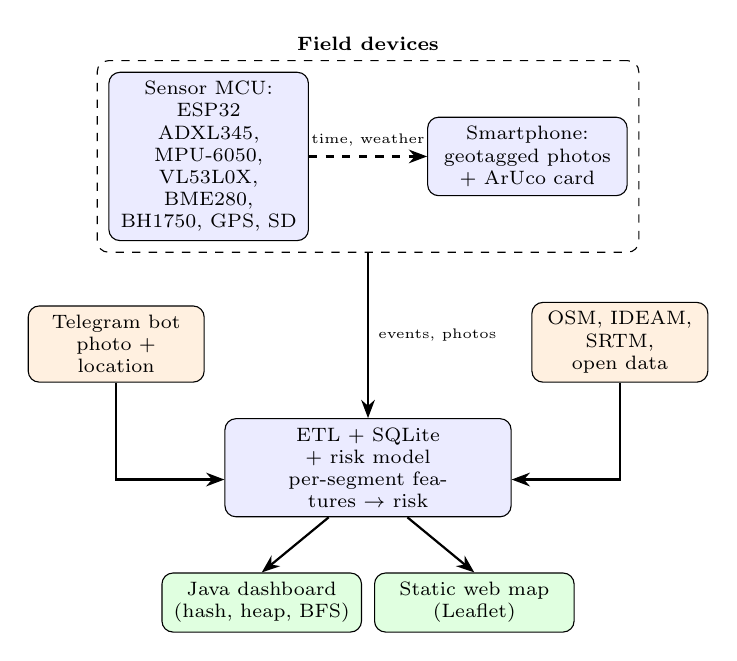
\begin{tikzpicture}[
  font=\scriptsize,
  blk/.style={draw, rounded corners, fill=blue!8, align=center, minimum height=0.8cm, text width=2.3cm},
  src/.style={draw, rounded corners, fill=orange!12, align=center, minimum height=0.8cm, text width=2.0cm},
  outb/.style={draw, rounded corners, fill=green!12, align=center, minimum height=0.75cm, text width=2.3cm},
  arr/.style={-{Stealth}, thick}
]
\node[blk] (sens) {Sensor MCU: ESP32\\ADXL345, MPU-6050,\\VL53L0X, BME280,\\BH1750, GPS, SD};
\node[blk, right=1.5cm of sens] (cam) {Smartphone:\\geotagged photos\\+ ArUco card};
\draw[arr, dashed] (sens) -- node[above, font=\tiny]{time, weather} (cam);
\begin{scope}[on background layer]
\node[draw, dashed, rounded corners, fit=(sens)(cam), inner sep=4pt, label={[font=\scriptsize\bfseries]above:Field devices}] (node) {};
\end{scope}
\node[blk, below=2.1cm of node.south, anchor=north, text width=3.4cm] (etl) {ETL + SQLite + risk model\\per-segment features $\rightarrow$ risk};
\node[src, left=0.25cm of etl.north west, anchor=south east, yshift=0.45cm] (cit) {Telegram bot\\photo + location};
\node[src, right=0.25cm of etl.north east, anchor=south west, yshift=0.45cm] (web) {OSM, IDEAM,\\SRTM, open data};
\draw[arr] (node.south) -- node[right, font=\tiny, align=left]{events, photos} (etl.north);
\draw[arr] (cit.south) |- ([yshift=-0.15cm]etl.west);
\draw[arr] (web.south) |- ([yshift=-0.15cm]etl.east);
\node[outb, below=0.7cm of etl.south, anchor=north, xshift=-1.35cm] (dash) {Java dashboard\\(hash, heap, BFS)};
\node[outb, below=0.7cm of etl.south, anchor=north, xshift=1.35cm] (map) {Static web map\\(Leaflet)};
\draw[arr] ([xshift=-0.5cm]etl.south) -- (dash.north);
\draw[arr] ([xshift=0.5cm]etl.south) -- (map.north);
\end{tikzpicture}
\caption{V\'IA VIVA architecture as implemented.}
\label{fig:arch}
\end{figure}

% =============================================================================================
\section{Data Acquisition}
\subsection{Sensors and Sampling}
The ADXL345 (\(\pm 16\)~g, full resolution, 3.9~mg/LSB \cite{adi_adxl345}) is the main sensor, sampled at 200~Hz. The sampling rate was set as a hypothesis (200~Hz, anti-aliasing near 80~Hz) and is validated from the power spectral density of the first drives: the lowest rate keeping 95\,\% of the energy is \pendiente{f\textsubscript{95} and minimum f\textsubscript{s} from the spectrum of real drives}. The MPU-6050 adds a gyroscope, the VL53L0X measures the distance to the pavement, and a NEO-6M GPS provides position, speed and UTC time. A BME280 (temperature, humidity and pressure; a DHT22 replaces it if only a BMP280 is available) and a BH1750 light sensor are read every 10~s and logged with GPS time to annotate the photo dataset. The first datasets were recorded with a phone (phyphox \cite{staacks2018phyphox}: accelerometer with gravity, gyroscope and GPS) at up to 30~km/h, following a written protocol (fixed mount, co-driver labeling); \pendiente{number of drives, km and labeled events}.

\subsection{Synchronization and Orientation}
Each event stores the UTC time of the last GPS fix and the milliseconds elapsed since it, so the ETL interpolates time and position. The node uses the orientation-free magnitude \(|a| - 1\,g\); the phone pipeline projects the dynamic acceleration on the gravity direction estimated with a 0.3~Hz low-pass filter.

\subsection{Threshold Detector and Maneuvers}
As requested by the Computer Architecture course, a threshold detector serves as the baseline and pre-labels drives. An event is declared when the GPS speed exceeds \(V_{\min}=5\)~km/h, the peak-to-peak vertical acceleration over 50~ms exceeds \(K=6\) times the background RMS (exponential average with \(\tau=2\)~s) and an absolute floor of 0.3~g, with a 1~s refractory period. The same rule is implemented in C on the node and in Python for pre-labeling. Gyroscope yaw rate (\(>15^\circ\)/s for 1~s) labels left and right turns, and longitudinal deceleration or a GPS speed drop (\(>2.5\)~m/s\(^2\)) labels hard braking, so that these maneuvers are not confused with potholes. These parameters are initial values: \pendiente{calibrated parameters and detector precision/recall on labeled drives}.

% =============================================================================================
\section{Computer Architecture of the Node}
\subsection{Buses and Pins}
The ADXL345 uses VSPI (native SCK/MISO/MOSI pins; chip select moved off the boot pin GPIO~5) with the ESP-IDF \texttt{spi\_master} driver and DMA. The microSD uses HSPI routed through the GPIO matrix, because the native HSPI pins include GPIO~12 and~15, which are boot-strapping pins (GPIO~12 selects the flash voltage). The matrix limits SPI to about 26~MHz, enough for the card at 10~MHz. The MPU-6050, VL53L0X, BME280 and BH1750 share I\textsuperscript{2}C at 400~kHz (the slow environmental sensors are read in the same task, so no bus lock is needed) and the GPS uses UART2. Removing the camera freed GPIO~25 and~35; GPIO~25 hosts the optional DHT22 one-wire line.

\subsection{FIFO, Interrupt and DMA Ping-Pong}
The ADXL345 FIFO works in stream mode with a watermark of 31 samples (the field has 5~bits), so the interrupt on GPIO~34 arrives every 155~ms at 200~Hz. The acquisition task (core~1, highest priority) queues one DMA transaction per FIFO entry at 1.5~MHz (below 1.6~MHz no extra delay is needed between FIFO reads) and fills one half of a ping-pong buffer while the processing task (core~1) works on the other; if processing lags, the lost block is counted. Wi-Fi, the web page, GPS, I\textsuperscript{2}C (motion and environment), microSD and statistics run on core~0.

\subsection{Experiments}
Table~\ref{tab:exp} lists the experiments, which the firmware logs to the microSD (\texttt{exp\_NNN.csv}); E2--E4 are measured at boot, before the application tasks start. The quantized network occupies 872~bytes against 3\,152~bytes in float32 (788 parameters). Measured results:

\begin{table}[!t]
\centering
\caption{Computer-architecture experiments implemented in the firmware.}
\label{tab:exp}
\footnotesize
\begin{tabularx}{\columnwidth}{@{}l>{\raggedright\arraybackslash}X>{\raggedright\arraybackslash}X@{}}
\toprule
\textbf{ID} & \textbf{Comparison} & \textbf{Metrics} \\
\midrule
E1 & Polling vs.\ per-sample interrupt vs.\ FIFO + DMA ping-pong & Lost samples, jitter, CPU load per core, current \\
E2 & Weights in flash (cached) vs.\ SRAM & Inference latency (first call and mean) \\
E3 & float32 vs.\ int8 (and random forest) & Latency, memory, agreement, F1 \\
E4 & I\textsuperscript{2}C (MPU-6050) vs.\ SPI (ADXL345) & Read time, \(\mu\)s per byte, CPU share \\
\bottomrule
\end{tabularx}
\end{table}

\incluirsiexiste{tablas/e1.tex}{E1 results (lost samples, jitter, CPU) measured on the node}
\incluirsiexiste{tablas/e2e3.tex}{E2/E3 inference latency measured on the node}
\incluirsiexiste{tablas/e4.tex}{E4 I$^2$C vs.\ SPI read time measured on the node}
\incluirsiexiste{tablas/corriente.tex}{node current measured with the USB tester}

% =============================================================================================
\section{Signal Processing and Edge AI}
For each detector trigger the node keeps a 2~s window (1.5~s before, 0.5~s after) and computes peak, RMS, kurtosis, crest factor, maximum jerk and the sign of the peak; the training pipeline replicates exactly this computation. Two classifiers are compared: a random forest (10 trees, depth \(\le 6\)) exported to C with emlearn \cite{emlearn,pedregosa2011sklearn}, and a 1-D convolutional network (two convolutions with 8 and 16 channels, global average pooling and a dense layer; 788 parameters) trained with PyTorch \cite{paszke2019pytorch} on 128 samples around the trigger. The network is quantized after training with symmetric per-tensor int8 scales \cite{jacob2018quant}: multiply-accumulate operations run in integers and only re-quantization uses a float multiplier; Python and C use the same rounding, so both produce identical outputs. All models are validated leave-one-drive-out, at window level and at event level over every detector trigger, against the threshold detector alone. Results: \pendiente{window F1 (forest, CNN float32, CNN int8) and event-level precision, recall, F1 and false positives per km vs.\ the threshold detector}.

% =============================================================================================
\section{Image Dataset and Classifier}
\label{sec:fotos}
\subsection{Collection Protocol}
Public road-image datasets do not cover Colombia \cite{arya2022rdd}, so the team builds its own. The target is at least 500 photos and 50 per class over nine classes: pothole, speed bump, crack, patch, manhole cover, obstacle, lane line, crosswalk and sound pavement, with a three-level severity for damage classes. At each site the phone (location on, JPEG, landscape, 1\(\times\) lens) takes four or five photos: context, front, side, a nadir view with the ArUco card, and the thermo-hygrometer display. Photos are taken at different times of day, light conditions, road classes and wet or dry surfaces, from the sidewalk and never by the driver, and are uploaded to a shared drive without messaging apps, which strip EXIF metadata. Collected so far: \pendiente{photos, sites and photos per class}.

\subsection{Ingestion and Metadata}
A Python pipeline reads JPEG and HEIC files, takes date, time and GPS from EXIF, derives the time of day, and assigns the nearest OpenStreetMap segment (\(\le 30\)~m) and its neighborhood. Temperature and humidity come, in this order, from the thermo-hygrometer reading, from the node log within \(\pm 30\)~min, or from an hourly historical weather API for Tunja \cite{openmeteo}, and daily rainfall from the nearest IDEAM station. Faces and plates are blurred with Haar cascades \cite{viola2001rapid} (face candidates must contain skin tones; without this check the detector fired on crosswalk stripes), EXIF is removed, and a quality report lists photos without GPS or date, blurred (variance of the Laplacian) or near-duplicate (difference hash from the same author within 2~min), and the count per class, time of day, light and road class. A local web tool lets two team members label class, severity, angle, light, wet surface and road class with keyboard shortcuts.

\subsection{Scale and Perspective}
A printed \(10\times10\)~cm card carries an ArUco marker \cite{garrido2014aruco} of 80~mm. Its four corners, refined to sub-pixel accuracy, define a homography \cite{hartley2004mvg} from the image to the pavement plane, which rectifies the photo to a nadir view at 1~mm per pixel; the damage is segmented as the largest dark region not touching the image border, and its area is reported in cm\textsuperscript{2}. The estimate refers to the opening of the damage in the pavement plane and fails with hard shadows or standing water. It is validated against length and width measured with a tape in the field (ellipse approximation): \pendiente{area error vs.\ tape measurements}.

\subsection{Classifier}
A MobileNetV3-Small \cite{howard2019mobilenetv3} pretrained on ImageNet is fine-tuned on \(224\times224\) inputs with augmentation and class weights. Train, validation and test sets are split \emph{by site} with stratified group folds: all photos of the same spot (within 15~m) fall on the same side, because a per-photo split would let the model recognize places instead of classes. The model is exported to TensorFlow Lite in float32 and with full-integer int8 post-training quantization \cite{jacob2018quant}, and the int8 model is evaluated on the same test set. The whole pipeline was verified end to end with synthetic images, which are flagged and never reported as results. Results: \pendiente{per-class precision, recall and F1, confusion matrix and macro-F1 for float32 and int8, model sizes}.

% =============================================================================================
\section{Data Structures}
The dashboard implements its own structures to analyze their complexity (Table~\ref{tab:ed}). A separate-chaining hash table (resized at load factor 0.75) stores the adjacency lists of the street graph (\NNodos{} intersections, \NTramos{} segments) and a geohash spatial index (precision~7, \(\approx\)153~m cells, segments registered in every cell they cross). A binary max-heap built in \(O(n)\) ranks segments by risk, and breadth-first search returns the corridor of a segment and the connected components of high-risk segments (candidate work orders). Measured on the real Tunja graph (2\,000 random queries), the geohash index compares 108 segments per nearest-segment query against 5\,775 by brute force (about 9~\(\mu\)s vs.\ 180~\(\mu\)s on the development laptop) and returns the same segment in every query. Loading the database and building all structures takes about 240~ms.

\begin{table}[!t]
\centering
\caption{Data structures of the dashboard and their cost.}
\label{tab:ed}
\footnotesize
\begin{tabularx}{\columnwidth}{@{}>{\raggedright\arraybackslash}X l l@{}}
\toprule
\textbf{Operation} & \textbf{Structure} & \textbf{Time} \\
\midrule
Segment by id & Hash table & \(O(1)\) avg. \\
Nearest segment to a click & Geohash + hash & \(O(1)+O(m)\) vs.\ \(O(n)\) \\
Top-\(k\) risk ranking & Binary heap & \(O(n + k\log n)\) \\
Corridor of a segment & BFS & \(O(V'+E')\) \\
High-risk zones & BFS per component & \(O(V+E)\) \\
\bottomrule
\end{tabularx}
\end{table}

% =============================================================================================
\section{ETL, Citizen Channel and Data}
The ETL downloads the drivable street graph of Tunja with OSMnx: \NNodos{} nodes and \NTramos{} undirected segments (\KmTramos~km); only \PctSuperficie\,\% of the segments have a surface tag in OSM (Fig.~\ref{fig:tunja}). Node elevations from SRTM 30~m \cite{farr2007srtm} give the slope of \NPendiente{} segments longer than 30~m (median \PendMediana\,\%, 90th percentile \PendPnoventa\,\%; Fig.~\ref{fig:pend}). Daily rainfall from \NEstaciones{} IDEAM stations within 15~km \cite{ideam_precip} (\LluviaDesde{} to \LluviaHasta) is interpolated to each segment by inverse distance weighting, and the \NBarrios{} neighborhoods and rural areas of the municipal open-data portal \cite{tunja_barrios} define the spatial groups. Scrapers respect \texttt{robots.txt} and a crawl delay. Drives are map-matched to the nearest segment (\(\le 25\)~m) and only the list of reviewed segments is kept, never the trajectory. Citizens report through a Telegram bot that stores a salted hash instead of the user identifier and answers with a report number and status. The full database is rebuilt from scratch by one PowerShell script (305~s in a clean copy).

\begin{figure}[!t]
\centering
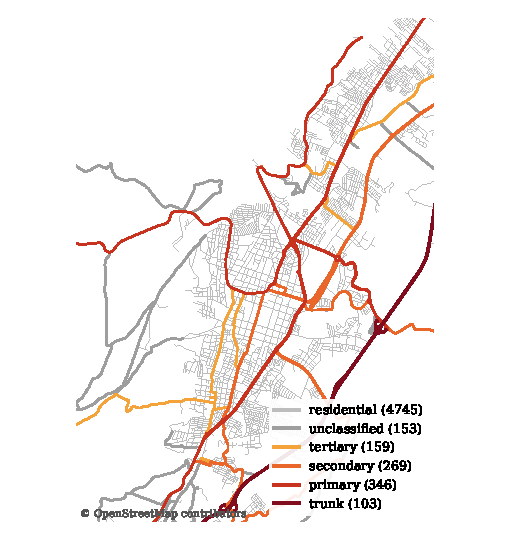
\includegraphics[width=\columnwidth]{figuras/tunja_tramos.pdf}
\caption{Drivable street graph of Tunja by road class (\NTramos{} segments; \copyright\ OpenStreetMap contributors).}
\label{fig:tunja}
\end{figure}

\begin{figure}[!t]
\centering
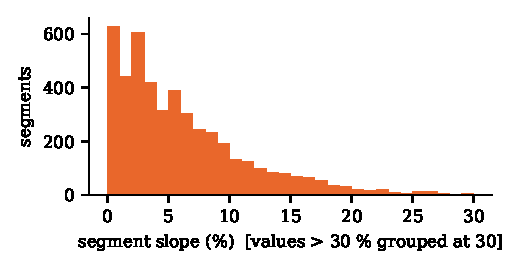
\includegraphics[width=\columnwidth]{figuras/pendiente.pdf}
\caption{Segment slope from SRTM 30~m (segments \(\ge 30\)~m).}
\label{fig:pend}
\end{figure}

% =============================================================================================
\section{Georeferenced Risk Model}
Each segment receives road class, surface, length, slope, 30-day and maximum daily rainfall, known hazards within 300~m on other segments (the segment's own hazards are excluded to avoid label leakage), crashes within 200~m, and measured roughness and depth. Labels are 1 for segments with a confirmed pothole and 0 for segments reviewed without one. Because municipal data had not arrived by \pendiente{date}, the model uses the agreed fallback (plan~B): segments reviewed in labeled drives and field visits plus pothole reports from the bot; each run records its label source. A logistic regression and a random forest are validated with group \(k\)-fold by neighborhood \cite{roberts2017cv}, reporting the spatial AUC (target \(\ge 0.70\)) next to a random-fold AUC to show the optimism of non-spatial validation. Results: \pendiente{number of labeled segments, spatial AUC of both models and label source}. Field validation compares the ten highest-risk unreported segments with ten random ones: \pendiente{segments with potholes in top-10 vs.\ random-10}.

% =============================================================================================
\section{Results Summary}
\begin{table}[!t]
\centering
\caption{Evaluation metrics: targets and measured values.}
\label{tab:metrics}
\footnotesize
\begin{tabularx}{\columnwidth}{@{}>{\raggedright\arraybackslash}X l l@{}}
\toprule
\textbf{Metric} & \textbf{Target} & \textbf{Measured} \\
\midrule
Pothole detection F1 (LODO) & \(\geq 0.80\) & \pendiente{F1} \\
False positives per km & \(\leq 1\) & \pendiente{FP/km} \\
Event position error & \(\leq 5\) m & \pendiente{m} \\
Inference latency per window & \(\leq 50\) ms & \pendiente{ms} \\
Lost samples under full load & 0 & \pendiente{E1} \\
Weights, int8 vs.\ float32 & smaller & 872 vs.\ 3\,152 B \\
Own photo dataset & \(\geq 500\); \(\geq 50\)/class & \pendiente{photos} \\
Photo classifier macro-F1, int8 (by site) & reported & \pendiente{F1} \\
Damage area error vs.\ tape & reported & \pendiente{\%} \\
Nearest-segment comparisons & \(\ll n\) & 108 vs.\ 5\,775 \\
Risk-model AUC (spatial CV) & \(\geq 0.70\) & \pendiente{AUC} \\
Top-10 risk vs.\ random & higher & \pendiente{field visit} \\
\bottomrule
\end{tabularx}
\end{table}
Table~\ref{tab:metrics} gathers the targets of the proposal. Only implementation figures are reported so far; every performance figure remains pending until it is measured.

% =============================================================================================
\section{Discussion and Limitations}
OpenStreetMap lacks surface information for most segments, neighborhoods are available as points (segments are assigned to the nearest point), and five rain gauges barely resolve spatial rainfall differences inside the city. The orientation-free magnitude \(|a|-1\,g\) on the node is simpler than projecting on gravity, at the cost of mixing lateral motion; the maneuver detector mitigates turns and braking. The VL53L0X loses range under strong sunlight. Map matching by nearest segment errs near intersections (in a synthetic test it recovered 26 of 28 segments with potholes). \pendiente{discussion of the measured results}.

Future work, outside the scope of this delivery: a laser grid module (structured light) to measure pothole depth, which could not be obtained in time; an optional read-only OBD-II link (ELM327 over Bluetooth) to use the vehicle speed as a backup for GPS; and automatic on-vehicle capture with a camera module, whose firmware is kept in the repository but removed from the design.

% =============================================================================================
\section{Ethical and Legal Considerations}
Faces and plates are personal data under Law 1581 of 2012 \cite{ley1581}: faces and plates in the photo dataset are blurred and EXIF metadata removed before analysis, photos are taken avoiding people and plates and are not published, citizen photos are not published, the bot stores only a salted hash of the user, and the system keeps events and lists of reviewed segments, not trajectories. V\'IA VIVA issues no fines \cite{ley1843}. Only sources that allow automated access are scraped, and municipal data requested by letter are not published without permission.

% =============================================================================================
\section{Conclusion}
V\'IA VIVA implements the full chain from an ESP32 sensor node with DMA-based acquisition and on-device int8 inference to a georeferenced risk model, a citizen bot, a dashboard and a public map, all reproducible from a single repository. \pendiente{conclusion with the measured detection and prediction results}.

\bibliography{referencias}

\end{document}
